\section{Experimental procedure}\label{sec:procedure}
In this experiment, we set up two detectors with equidistant from the source. Distance from detector to source is \SI{5}{\cm} for both detectors, as suggested by tutor. This ensures precision within the limited time frame.

Fast and slow signals circuits are separate readout from detectors. Both of them get combined in to an universal counter (UC) through a gate and delay ($\text{G}^{2}-\text{D}^{2}$). Two CFDs are connected to filter out zero crossing in fast signal circuit and two amplifiers are connected in slow signal circuit. Three delays are used, two in slow signal circuit (built-in in SCA) and one between CFD2 and FC. A timer connected with all counters to fixed the counting time. The figure~\ref{fig:CCuit} shows a schematic of the set and the tasks we did on this experiment are described in the following. Detector part in real life is shown in \ref{fig:detect}.
\begin{figure}[ht]
	\centering
	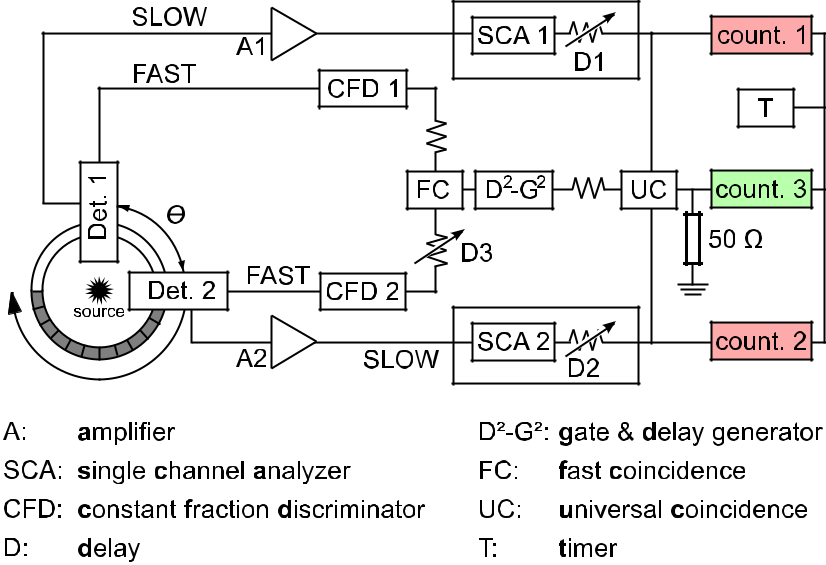
\includegraphics[width=0.7\linewidth]{./figs/CirCuit.png}
	\caption{Set up of fast and slow coincidence circuit~\cite{descr}.}%
	\label{fig:CCuit}
\end{figure}
\begin{figure}[ht]
	\centering
	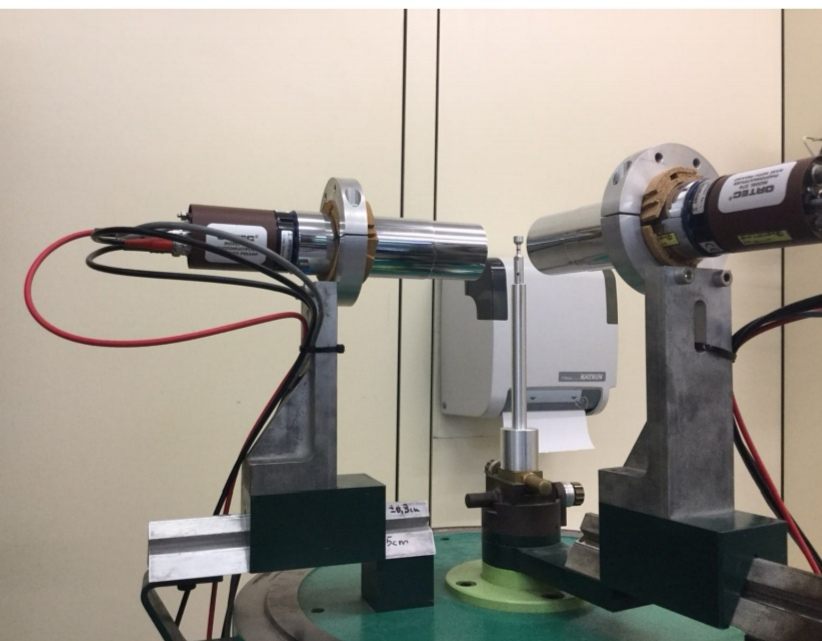
\includegraphics[width=0.4\linewidth]{./figs/detectors.jpg}
	\caption{Set up of two detectors where one is fixed and another one is movable to rotate at a fixed radial distance from the fixed detector.}%
	\label{fig:detect}
\end{figure}

\subsection{Adjusting the gain of the Amplifier}
First, we adjusted the gain of both amplifiers  ($\text{A}_{1}$ and $\text{A}_{2}$) during the set up of the experiment. The amplifiers output is linear up to $V_\text{max}=\SI{9}{\volt}$. With oscilloscope the amplifications of amplifiers are set to obtain a signal without saturation. Here we took gains of the amplifiers as much as possible. Signals get saturated if signals have a clear plateau. 
\begin{figure}[ht]
	\centering
	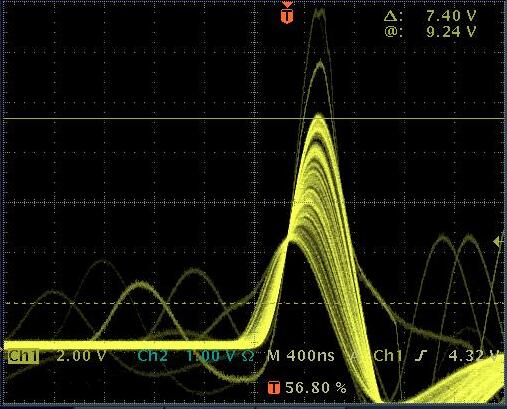
\includegraphics[width=0.6\linewidth]{./figs/Amplifier.jpg}
	\caption{Amplified signal output from the detector. The other output looks the same.}%
	\label{fig:Amplified}
\end{figure}

\subsection{Adjusting of the CFD}
\begin{figure}[H]
	\centering
	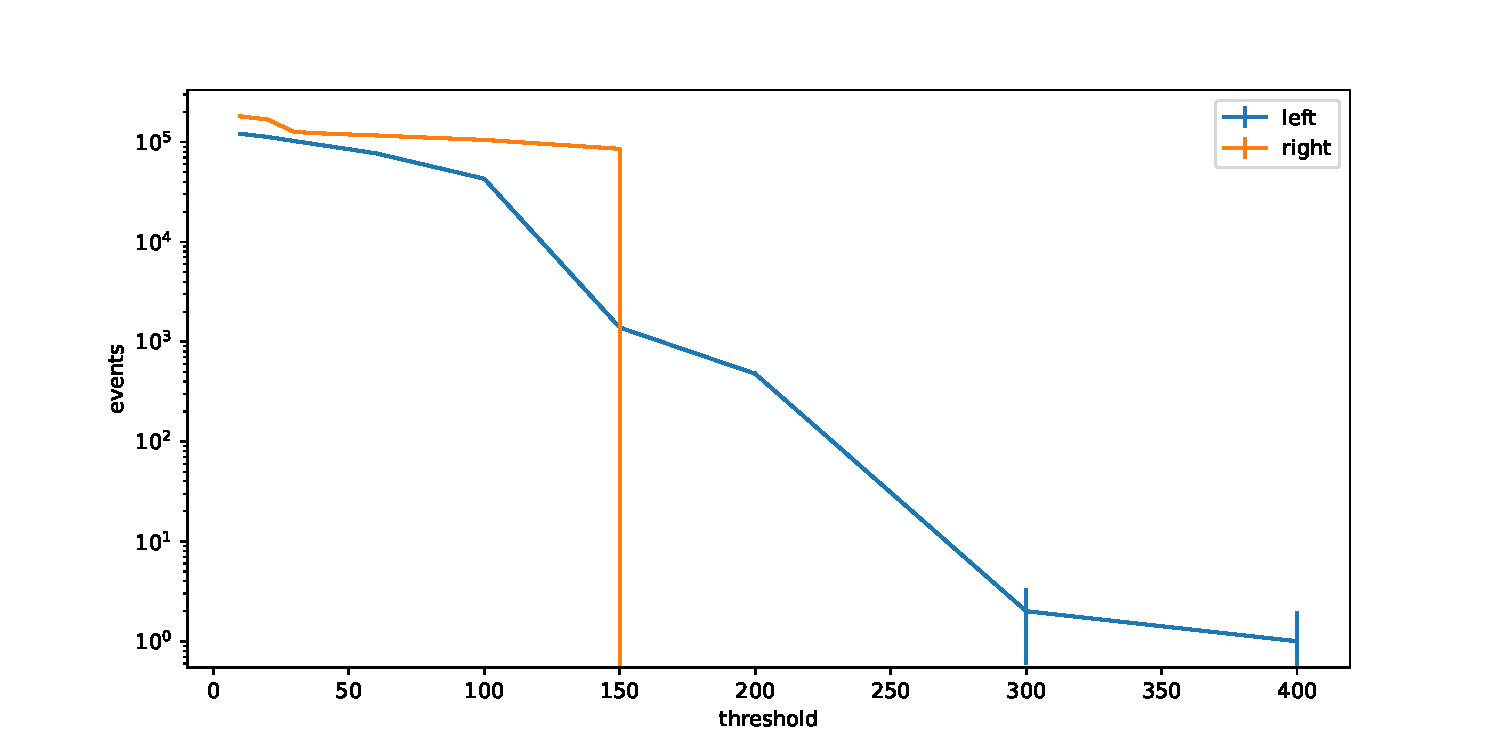
\includegraphics[width=0.8\linewidth]{./figs/cfd.pdf}
	\caption{Number of events with source. Note vertical axis used log-scale.}%
	\label{fig:Cfd1}
\end{figure}
\begin{figure}[ht]
	\centering
	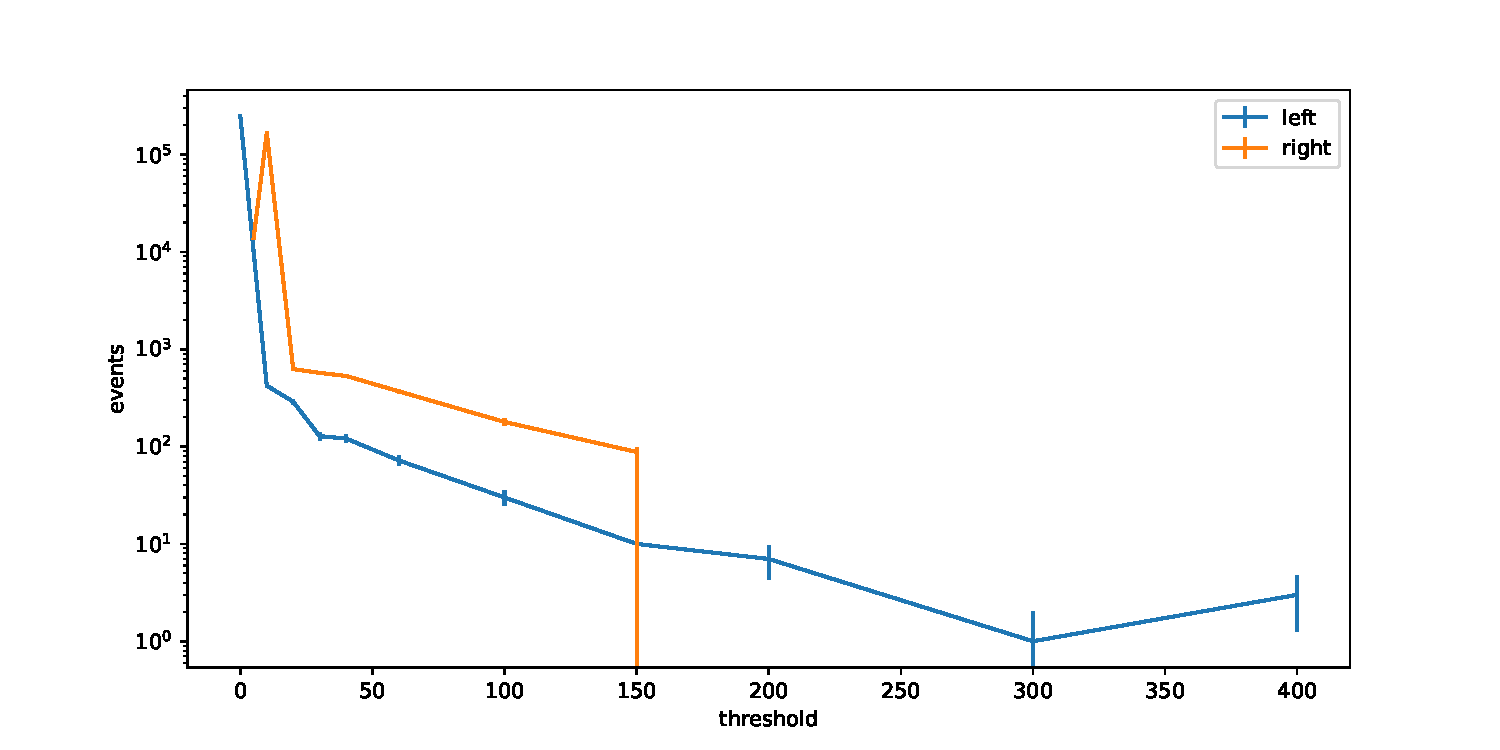
\includegraphics[width=0.8\linewidth]{./figs/cfd2.pdf}
	\caption{Number of events without source. Note vertical axis used log-scale.}%
	\label{fig:Cfd2}
\end{figure}

CFD has a threshold-discriminator which helps to filter out zero crossing that belongs to electronic noise and not to a true scintillation signal~\cite{descr}. Performing a threshold scan allows to search out the right compromise. For that, CFD has restriction upon the minimum and maximum signals.  

Thresholds of CFD should be adjusted to detect only true signals, not the background noise signals. In that step, the negative outputs of the both CFDs are connected to the counters and the events are counted with and without source. Figure~\ref{fig:Cfd1} and~\ref{fig:Cfd2}, respectively, show the number of events with and without inserting source. Errors are calculated with $\Delta N \approx \sqrt{N}$.

Number of events without source contain only random events, aka backgrounds. With source it contains both signals and backgrounds. Figure~\ref{fig:Cfd1} has quite drastic drop in number of events, whereas in figure~\ref{fig:Cfd2} the drop is rather continuous after \num{30} or so. In the end, we set the threshold to \num{30}, since most random events are cut and wanted signals are still basically untouched.

\subsection{Setting up the Fast Coincidence}
Here we want to make sure that true coincidences arrive at same time (within resolving time of coincidence unit, to be precise). First, we connected both CFDs to the oscilloscope and triggered on the first channel signals. Then, on the second channel, true coincidence pulses are concentrated in small region. The random events are not the events we are looking for. 

We inserted a fixed delay into one of the fast branches and a variable delay into the other one, so that we can see the full prompt curve. Then, the CFDs are connected to the fast coincidence unit and the count rates are measured for different (variable) delay with resolving time \SI{25}{\nano\s}. 

\begin{figure}[H]
   \centering
   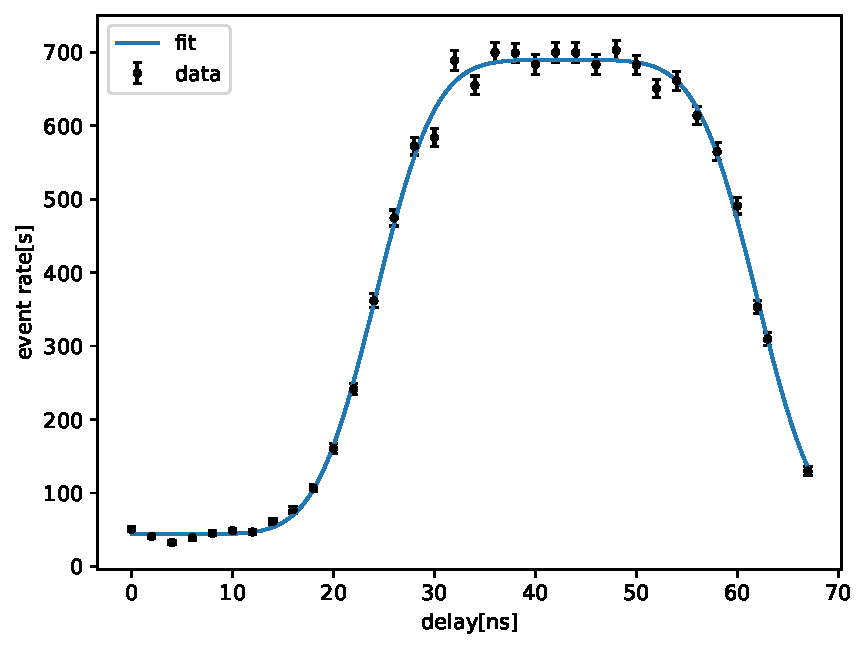
\includegraphics[width=0.6\linewidth]{prompt.pdf}
   \caption{Prompt curve}%
   \label{fig:prompt}
\end{figure}
Indeed, the prompt curve looks like a box with smeared egdges as stated in~\cite{descr}. Data points are fitted wit function
\begin{equation}
   f(t) = A_0 + A_1 \left( \frac{1}{2} + \erf \left(\frac{t-t_0}{\sigma} \right) \cdot \erf \left(\frac{t_1 - t}{\sigma} \right) \right)
\end{equation}
This is reasonable considering that signals are gaussian. Data and fit curve can be found in figure~\ref{fig:prompt}.

These parameters each represent something physical of the experiment: $A_0$ random coincidence since with extreme low/high delay the true coincidences don't safisfy the conincidence criteria, $A_1$ related to source intensity and detector efficient, $t_i$ resolution of corresponding detector, $\sigma$ resolving time of coincidence unit. Thus the width of the plateau depends on $\sigma$. This can be easily understood as if we turn up the resolving time, then there will more events considered as coincidences. The slopes are related to detector (time) resolutions, since it smears the CFD's logic output timing. Parameters from fitting are
\begin{align*}
   t_0 &= \SI{24.151 +- 0.151}{\nano\s} \\
   t_1 &=  \SI{61.949 +- 0.152}{\nano\s} \\
   A_0 &= \SI{205.436 +- 3.823}{\per\s} \\
   A_1 &= \SI{323.007 +- 3.580}{\per\s} \\
   \sigma &= \SI{6.612 +- 0.242}{\nano\s}
\end{align*}
Correlations of parameters are quite small, since the off-diagonal entries of covariance matrix are at least one magnitude lower. Thus correlations are neglected.

Shape of the prompt curve will change to basically flat (constant count rate) if the resolving time is chosen too short or too long: either no signals will be picked up or every pair of inputs will be counted as coincidence.

\subsection{Setting up the Slow Coincidence}
Again timings of output of fast coincidence and two SCAs need to be aligned. SCAs have built-in delays. With oscilloscope, signals are properly aligned with leading edges. It often gives us maximal overlap as well. In figure~\ref{fig:slow} the peaks are correctly aligned with each other.
\begin{figure}[ht]
	\centering
	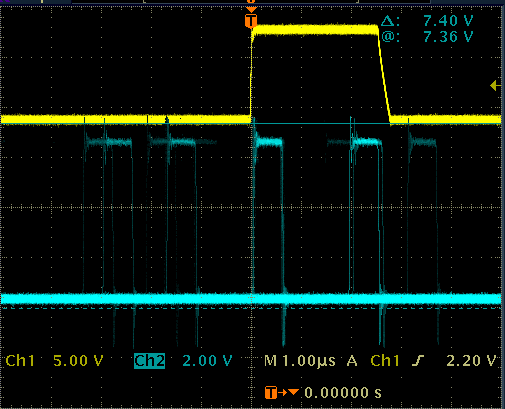
\includegraphics[width=0.5\linewidth]{./figs/slow.png}
	\caption{The timing alignment of signals from FC and two SCAs.}%
	\label{fig:slow}
\end{figure}


\subsection{Calibrating the Signal Channel Analyzer}
The SCAs are used to select the energy deposited in the detector. In this step, we performed the energy calibration and recorded the energy-spectrum by using SCAs. For that the SCAs are set to their window mode. Window size is kept constant due to normalization. We want to see all structures of energy spectrum, so $20$ window width is selected. 

For lower statistical error, events are counted until roughly $1\%$ precision is reached. Figure~\ref{fig:sca1} shows the energy spectra. Quite awful in this plot is that second peak of right signals doesn't appear. The SCA windows should be set to include both photopeaks for higher coincidence rate. So amplification of right slow circuit is lowered. Figure~\ref{fig:sca2} shows energy spectra after we readjusted amplification. In the end, SCA windows are set to $[720, 960]$.
\begin{figure}[ht]
	\centering
	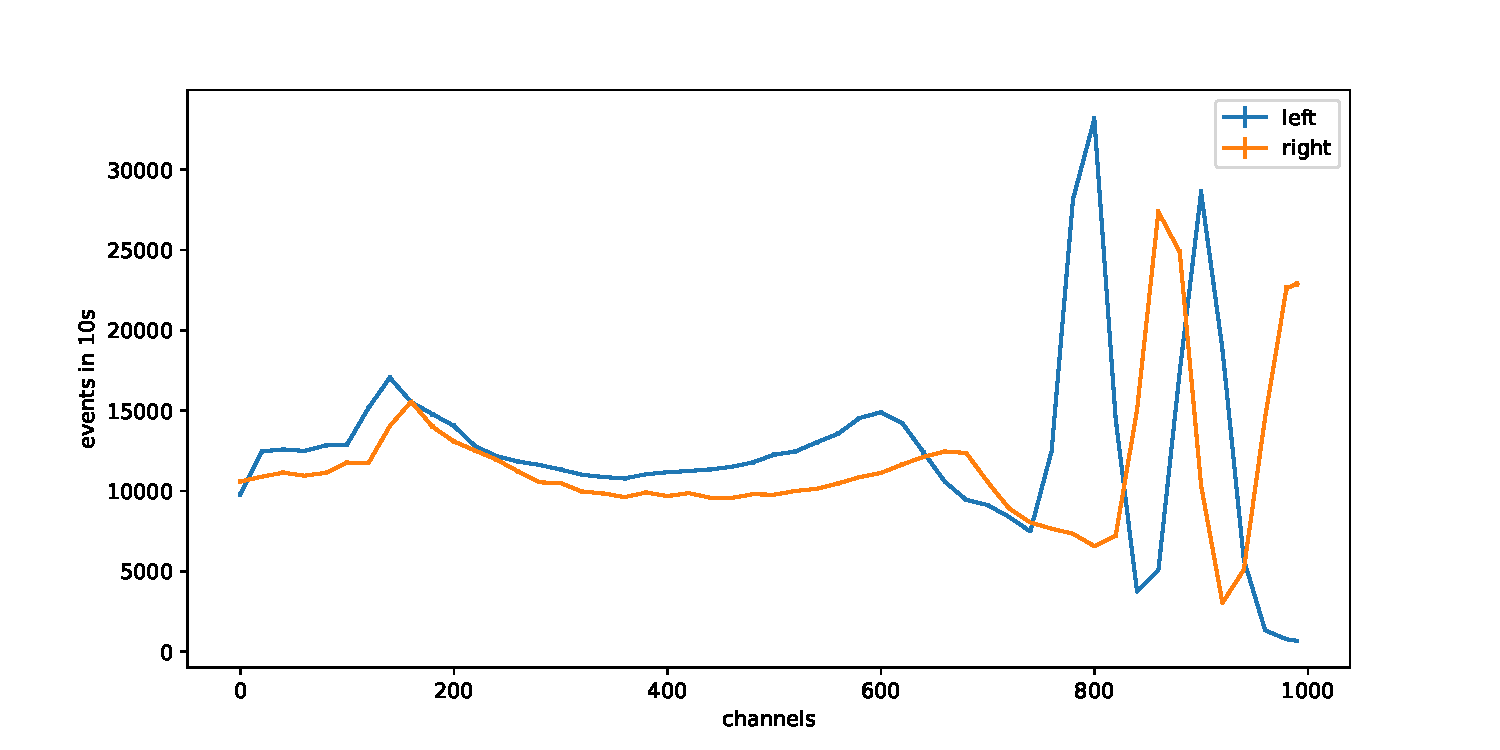
\includegraphics[width=0.7\linewidth]{./figs/sca.pdf}
	\caption{The energy spectra.}%
	\label{fig:sca1}
\end{figure}
\begin{figure}[ht]
	\centering
	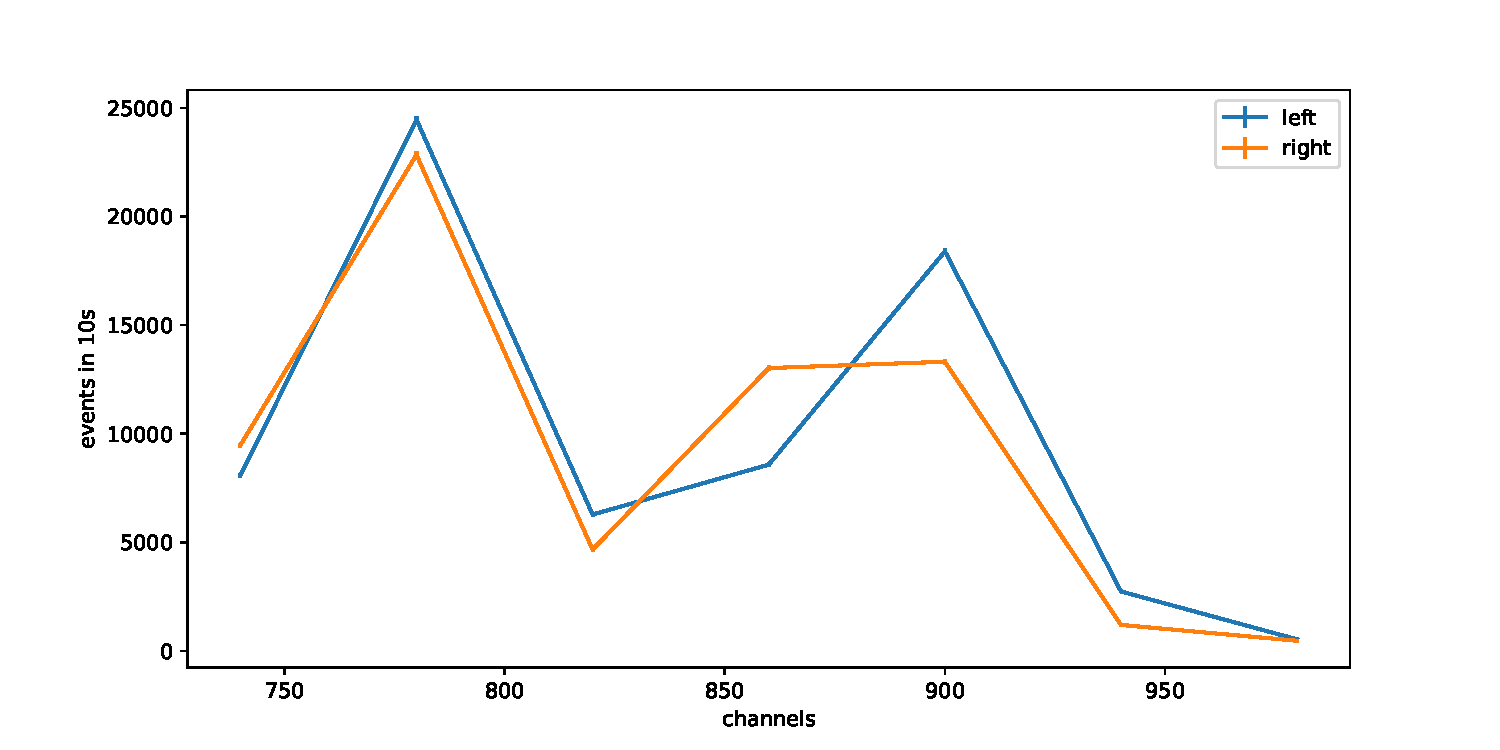
\includegraphics[width=0.7\linewidth]{./figs/sca2.pdf}
	\caption{The energy spectra after readjusting amplification. }%
	\label{fig:sca2}
\end{figure}

\subsection{Main Measurement}
After adjusting all the involving apparatus in the experiment, we stated to perform the main measurement of the experiment. The count rates are measured for different angles between these two detectors. We have taken firstly some measurements with larger steps and longer duration, then some measurements with smaller steps and shorter duration.  Throughout whole experiment, measurement at \SI{180}{\degree} is repeated three times in order to have knowledge of setup stability and systematic errors.

In the end, an extra measurement of random coincidence is carried out, where the variable delay in fast branches is turned all the way up, so that true coincidences are not counted. The random coincidence rate is
\begin{equation}
   \dot{R} = \SI{2.218 +- 0.061}{\per\s}
   \label{math:random}
\end{equation}
Delays of SCAs remain unchanged. This would not have big impact on measurement of random coincidence, since only fast circuit has accurate timing information.

Random coincidence rate can also be calculated. Assuming extremely narrow signal peak (but still can be seen by fast circuit) and uniformly distributed signals, random coincidence rate is then the rate of two signals falling within resolving time.  It is given as~\cite{melissinos}
\begin{equation}
   \dot{R}_\text{pred} = \dot{N}_1 \dot{N}_2 \Delta t = \SI{1.643 +- 0.013}{\per\s}
\end{equation}
Ideally the count rates are same for both detectors $\dot{N}_1 = \dot{N}_2$, but as we will see, there is misalignment. Count rates measured in main measurements are used here and their mean and standard deviation are calculation, since there are more than one set of data. Resolving time is again $\Delta t = \SI{25}{\nano\s}$. Errors are propagated properly.

This doesn't match measured value. It could imply that there some systematic error in electronics. But also the assumption could not be valid. Here we see that random coincidence, a source of background, is proportional to resolving time. In figure~\ref{fig:prompt}, the plateau is still quite long. In principle, the resolving time can still be lowered so that true coincidence doesn't get affected but random coincidence gets reduced.
\clearpage
